%!TEX program = pdflatex

\documentclass{UDEbeamerEN}

\usepackage{ifluatex}
\ifluatex
  \usepackage{fontspec}
  \usepackage{polyglossia} % babel replacement for use with fontspec
  \setdefaultlanguage[variant=american]{english}
  \selectlanguage[variant=american]{english}

  \setmainfont[Ligatures=TeX]{Linux Biolinum O}
  %\setmathfont[math-style=ISO,bold-style=ISO,vargreek-shape=TeX,Ligatures=TeX]{TeX Gyre Pagella Math}

  \usepackage{unicode-math} % fixes math
  \usepackage{lualatex-math} % fixes amsmath/mathtools ... for luatex

\else
  \usepackage[utf8]{inputenc}
  \usepackage[T1]{fontenc}
  \usepackage[american]{babel}
  \usepackage{libertine}
  \usepackage{microtype}
  \usepackage{amssymb}
  \usepackage{mathtools}
\fi

\usepackage[acronym, nomain, nowarn]{glossaries}
\loadglsentries{acronyms}

\usepackage{csquotes}
\usepackage[load-configurations={abbreviations,binary}]{siunitx}
\sisetup{load-configurations = abbreviations,binary-units, range-phrase = {\text{~to~}}, per-mode=fraction}
\usepackage{multirow}
\usepackage{tabu}
\usepackage{booktabs}
\usepackage{algorithmic}
\usepackage{algorithm}
\usepackage{url}

\usepackage{multimedia} % WARNING: \movie command does not seem to work with lualatex; use pdflatex instead
%\usepackage{xmpmulti}
\usepackage{media9}

\usepackage[defernumbers=true, style=alphabetic, citestyle=alphabetic, backend=biber, doi=false, url=false, block=ragged, maxnames=6]{biblatex}
\addbibresource{literature.bib}

\hypersetup{colorlinks=false}

\addtobeamertemplate{footnote}{}{\vspace{5ex}}


\title{A Comprehensive End-to-End Lag Model for Online and Cloud Video Gaming}
\author{Florian Metzger, Albert Rafetseder, Christian Schwartz}
\webadresse{https://www.mas.wiwi.uni-due.de/en}
\lehrstuhl{Modeling of Adaptive Systems}
\date[]{2016/08/29}

\def\Put(#1,#2)#3{\leavevmode\makebox(0,0){\put(#1,#2){#3}}}

\begin{document}


\frame{\titlepage}




\begin{frame}
	\frametitle{Games and Frames}
	%\framesubtitle{QoS and QoE of TCP Streaming in Mobile Networks?}
	\vspace{-0.5cm}

% clip generation:
% download source with youtube-dl
% ffmpeg -i csgo.mp4 -ss 00:24:24 -t 00:00:08 -an -vcodec copy clip1.mp4
% ffmpeg -i clip1.mp4 -vf "select=not(mod(n\,6))" clip1_6.mp4 
% ffmpeg -i clip1_6.mp4 -pix_fmt yuv420p clip1_6.mov 

	\begin{overprint}
		\only<1>{
			\begin{center}
				{\small CS:GO gameplay at 30fps (normally played at 120+)}\\
				\movie[width=9cm, height=6cm, repeat=true, poster]{}{clip1.mov}\\
				{\tiny clip extracted from \url{https://www.youtube.com/watch?v=02I5vVxlJhU}}
			\end{center}}
		\only<2>{
			\begin{center}
				{\small same clip at 6fps}\\
				\movie[width=9cm, height=6cm, repeat=true, poster]{}{clip1_6.mov}\\
				{\tiny clip extracted from \url{https://www.youtube.com/watch?v=02I5vVxlJhU}}
			\end{center}}
	\end{overprint}
\end{frame}

\begin{frame}
	\frametitle{Motivation and Past Issues}

	\begin{itemize}
		\item Increasing research interest for (networked) video game QoS and QoE
		\item Increasing focus on and demands of \textbf{competitive games}
		\item But many past endeavors treated video games similar to video streaming and faced issues
			\begin{itemize}
				\item Insufficient framerates (actual examples: \SI{3}{\hertz}, \SI{7}{\hertz}, \SI{15}{\hertz})
				\item Wrong choice of metrics (e.g. time-scale wise)
				\item Studies focused only on network delay, not E2E lag
				\item Observation periods too short
				\item No understanding of core gameplay mechanics
				\item Cannot generalize results from individual games to a whole ``genre''
			\end{itemize}

		\item Many interlocked mechanics in play
		\item Need for a better understanding of these mechanics
		\item Looking only at authoritative client/server games here, not peer-to-peer
	\end{itemize}

\end{frame}



\begin{frame}
	\frametitle{Frame- and Tickrates}

	\begin{block}{Framerate and Frametime}
		Rate at which the game renders distinct images. Frametime is the time between two such images.
	\end{block}

	\pause
	\begin{block}{Tickrate}
		Rate at which the server in a client/server-game updates its game simulation state.
	\end{block}


	\pause
	\begin{columns}[T]
		\column{0.5\textwidth}
			\begin{center}
				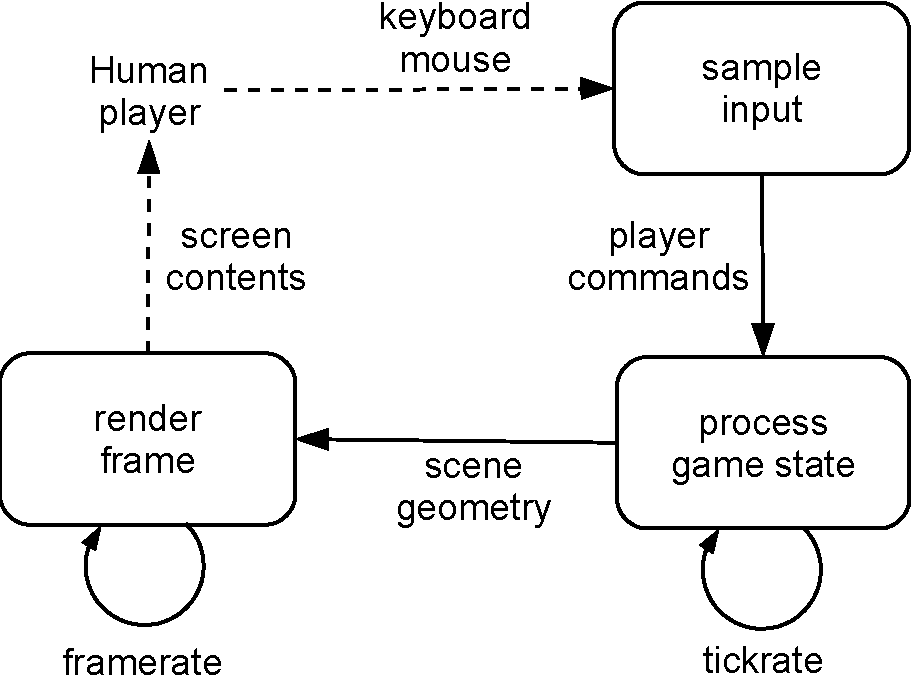
\includegraphics[width=0.7\columnwidth]{../../../models/game_loop.pdf}
			\end{center}

		\pause
		\column{0.5\textwidth}
			\vspace{-1mm}
			Framerate constraints:
			\vspace{-1mm}
			\begin{itemize}
				\item Motion perception in video: Based on principle of apparent motion according to \cite{wertheimer1912experimentelle}starting at a min. frame rate of \SI{16}{\hertz}
				\item But framerate and tickrate are also governing factors for input latency

				\item Common game frame rates:\\ \SI{30}{\hertz}, \SI{60}{\hertz}, \SI{120}{\hertz}, \SI{144}{\hertz}
				%\item Reasoning: display refresh rates: lock to certain fractions of monitor refresh rate, else VSYNC or tearing issues
			\end{itemize}
	\end{columns}

\end{frame}


\begin{frame}
	\frametitle{Information Deficit through Low Framerate}
	\framesubtitle{Low framerates are a source of lag}

	\begin{center}
		%ffmpeg -f gif -i eli5-framerate.gif -pix_fmt yuv420p eli5-framerate.mov
		\movie[width=9cm, height=6cm, repeat=true, poster]{}{extras/framerate.mov}\\
		{\tiny\url{http://blog.logicalincrements.com/2015/04/does-fps-matter-decide-for-yourself/}}
	\end{center}
\end{frame}


\begin{frame}
	\frametitle{What is End-to-End Lag?}

	\begin{itemize}
		\item Perceived delay or inconsistency from an input action to the reaction
		\item Caused by various latency sources, e.g. network QoS, I/O devices, game engine, game mechanics
		\item But also through the interplay of Sometimes caused by game mechanics
		\item Examples of tickrates in c/s-games: CS:GO \SIrange{64}{128}{\hertz}; Dota 2 \SI{30}{\hertz}; Overwatch \SI{60}{\hertz}
		\item Command message and client update message rates may also differ from tick- and framerate
	\end{itemize}
		\vspace{-4mm}
		\begin{center}
		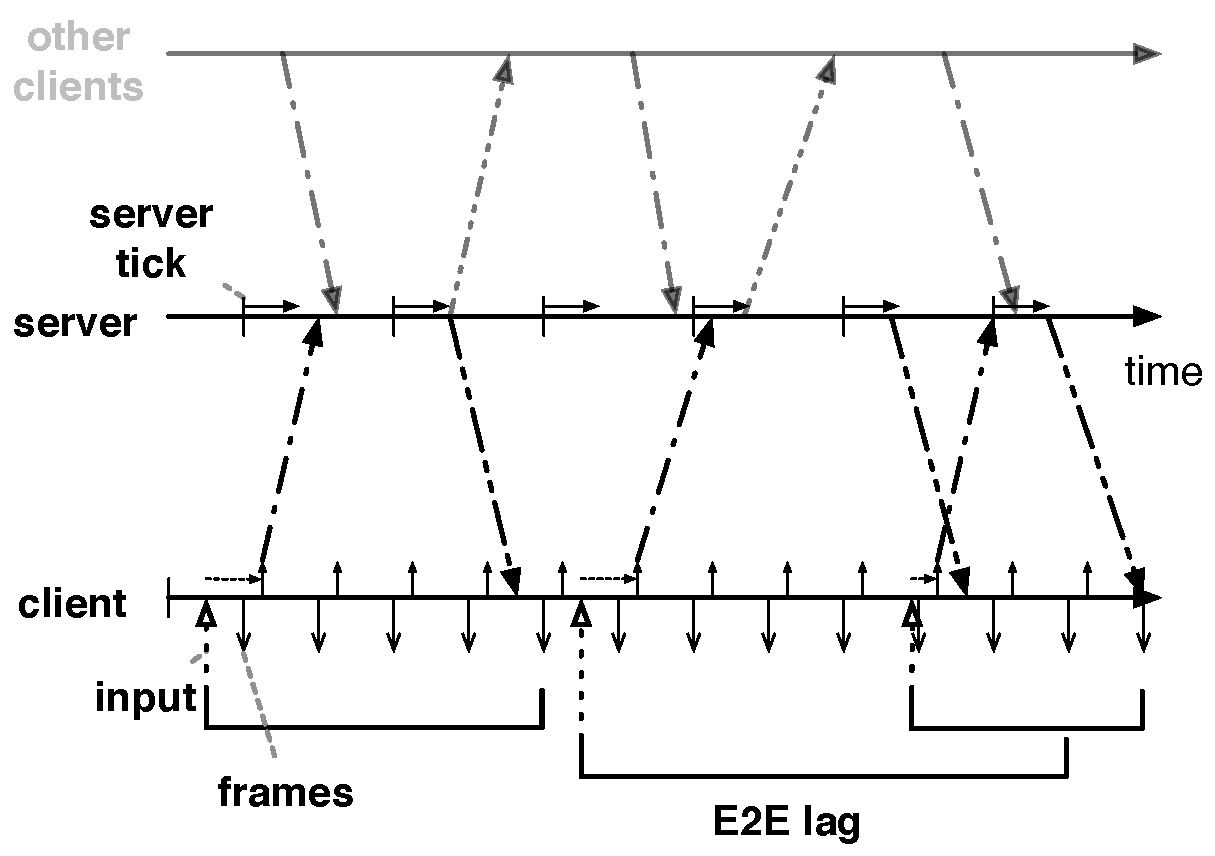
\includegraphics[height=4cm]{../../../models/tickrate-timeseries-poster.pdf}
	\end{center}

\end{frame}


\begin{frame}
	\frametitle{Attributes and Measures of Lag}

	\begin{itemize}
		\item Lag affects reaction and timings, gameplay, player performance 
		\item[$\Rightarrow$] potentially largest \textbf{QoE} influencer
		\item Every game is influenced differently by lag and exhibits a distinct lag profile
		\item Different viewpoints observe different lags, full E2E lag can only be captured externally
	\end{itemize}

	\begin{center}
		\vspace{-2mm}
		%Location of three measurement approaches to capture end-to-end lag

		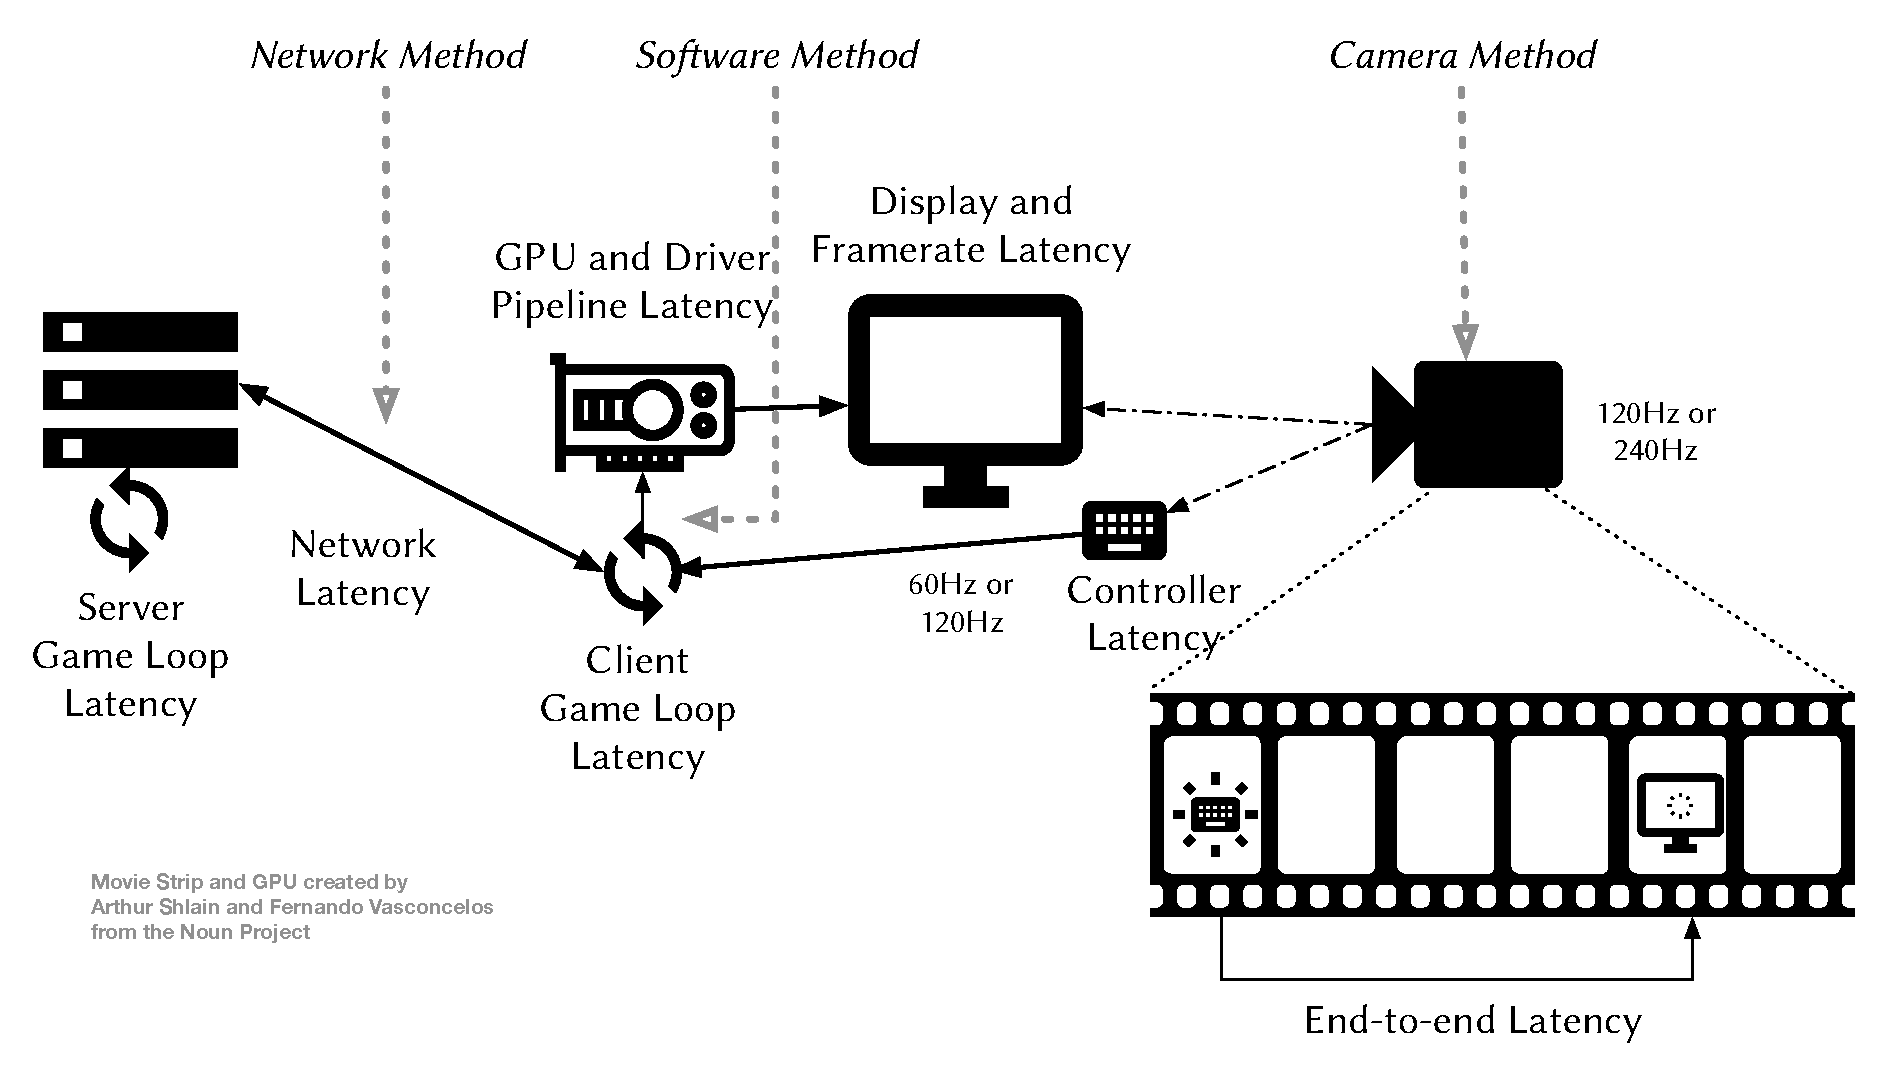
\includegraphics[height=4cm]{../../../models/e2e-lag.pdf}
	\end{center}

\end{frame}


\begin{frame}
	\frametitle{Modeling and Simulating Lag}

	\begin{itemize}
		\item End-to-End lag sources modeled as a queuing system
		\item Goal: investigate alternate lag sources not typically attributed to lag: frame- and tickrate, message rates, input and display devices
		\item Critical factor: interaction of multiple, independently clocked processes
	\end{itemize}

	\begin{center}
		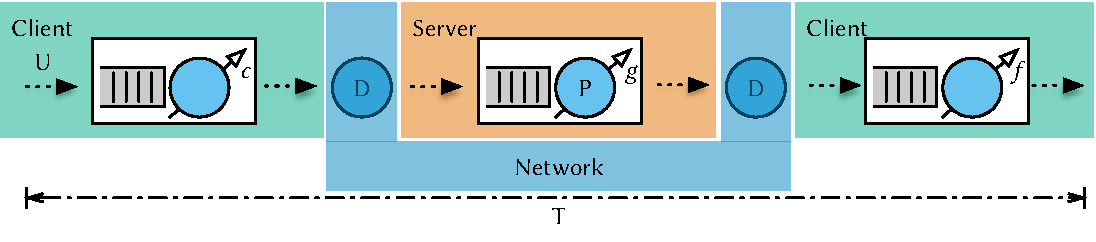
\includegraphics[height=2cm]{../../../models/e2e-lag-model.pdf}
	\end{center}

	\begin{itemize}
		\item Implemented as R simulation\footnote[frame]{\url{https://github.com/mas-ude/onlinegame-lag-sim}}
		\item Evaluated for several scenarios and parameter combinations
	\end{itemize}

\end{frame}


\begin{frame}
	\frametitle{Model Limitations and Caveats: Lag-Concealing Features in Games}

	Features that can reduce lag impact in games, not considered in the model

	\begin{columns}[T]
		\column{0.5\textwidth}
			\begin{itemize}
				\item Immediate visualization through client-side prediction of object actions (e.g. player movement) (without waiting for authoritative answer)
				\item Visualization interpolation between snapshots // extrapolation from last two server game state snapshots
				\item Lag compensation by doing hit detection on object positions slightly in the past
			\end{itemize}
		\column{0.5\textwidth}
			\vspace{-1mm}
			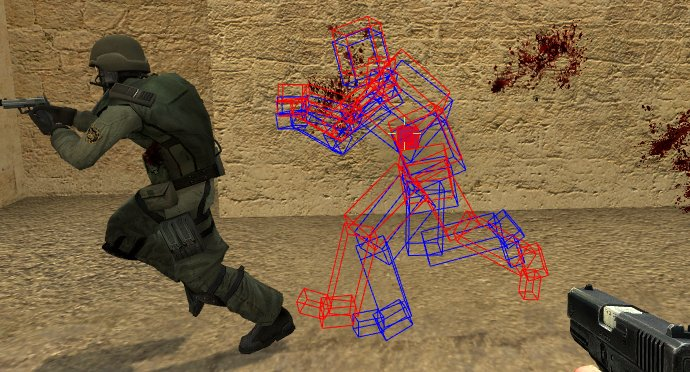
\includegraphics[height=3cm]{Lag_compensation.jpg}\\
			{\tiny\url{developer.valvesoftware.com/wiki/Lag_compensation}}
	\end{columns}

\end{frame}



\begin{frame}
	\frametitle{Results: Local Game}

	\begin{center}
		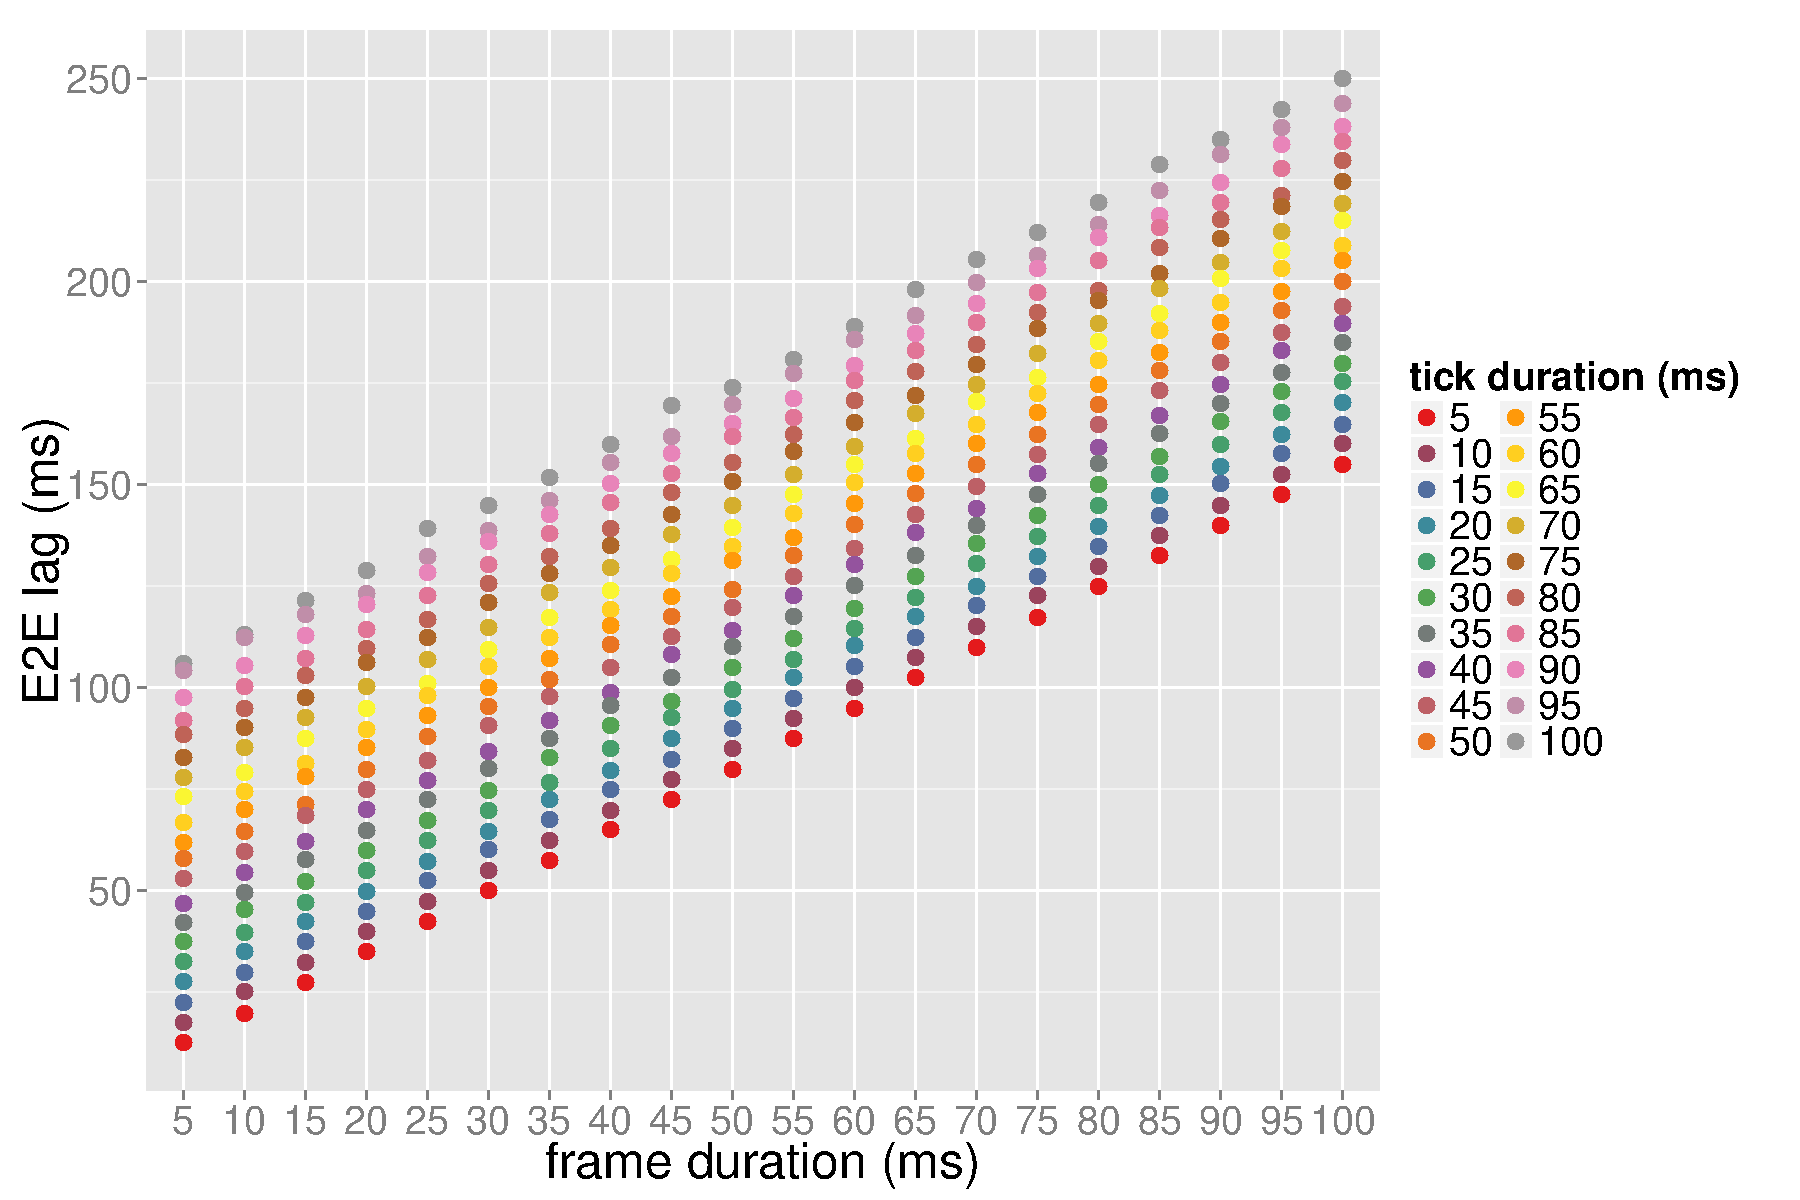
\includegraphics[height=5cm]{../../../simulation/visualization/nwless-onlinegame-1000rounds.pdf}

		Median \gls{E2E} lag under various frame and tick durations for a local game. Lower lag values are achieved at lower frame and tick durations; the frame duration has a larger influence on the \gls{E2E} lag.
	\end{center}
\end{frame}


\begin{frame}
	\frametitle{Results: Networked Game}

	\begin{center}
		\vspace{-9mm}
		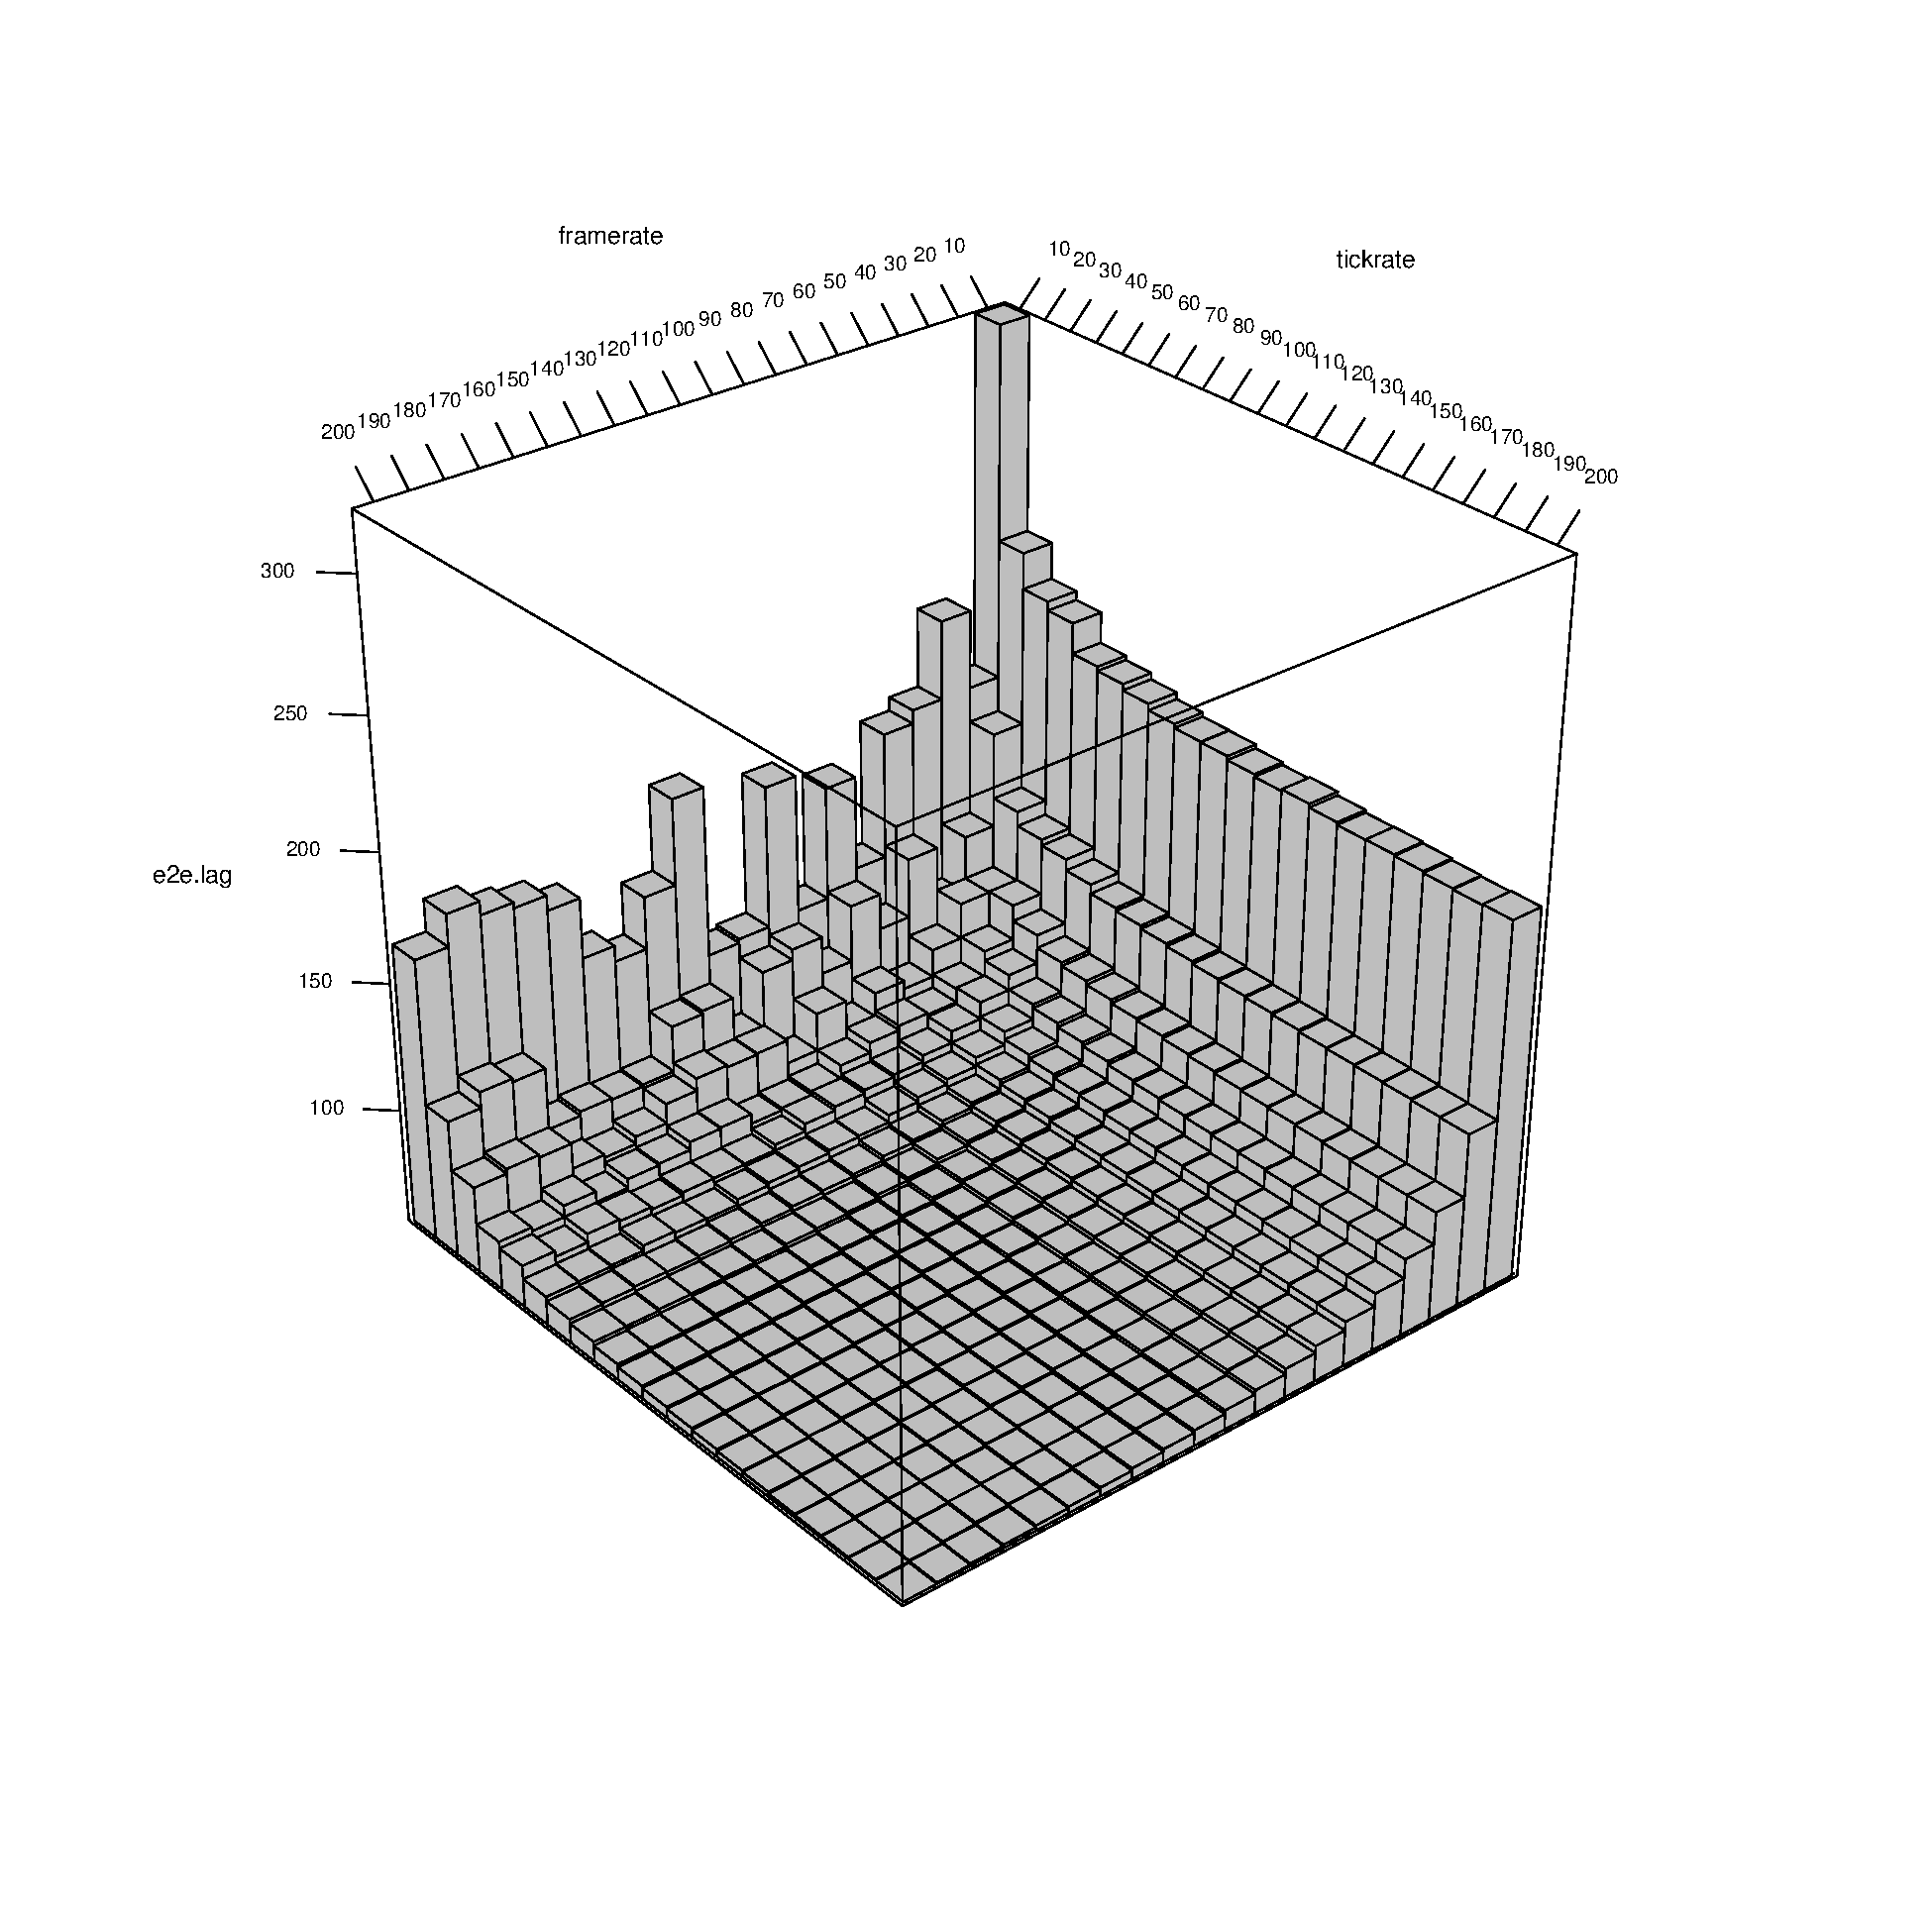
\includegraphics[height=5cm]{../../../simulation/visualization/e2e-lag-3dbars.pdf}
		\vspace{-10mm}
	\end{center}

	\begin{itemize}
		\item Networked game at \SIrange{10}{200}{\hertz} frame- and tickrates; median of $1000$ rounds for each bar
		\item \SI{40}{\milli\second} base network RTT
		\item Large influence of frame-/tickrate on E2E lag
		\item Negligible network influence at low frame-/tickrates
	\end{itemize}

\end{frame}


\begin{frame}
	\frametitle{Results: Cloud Game}

	\begin{center}
		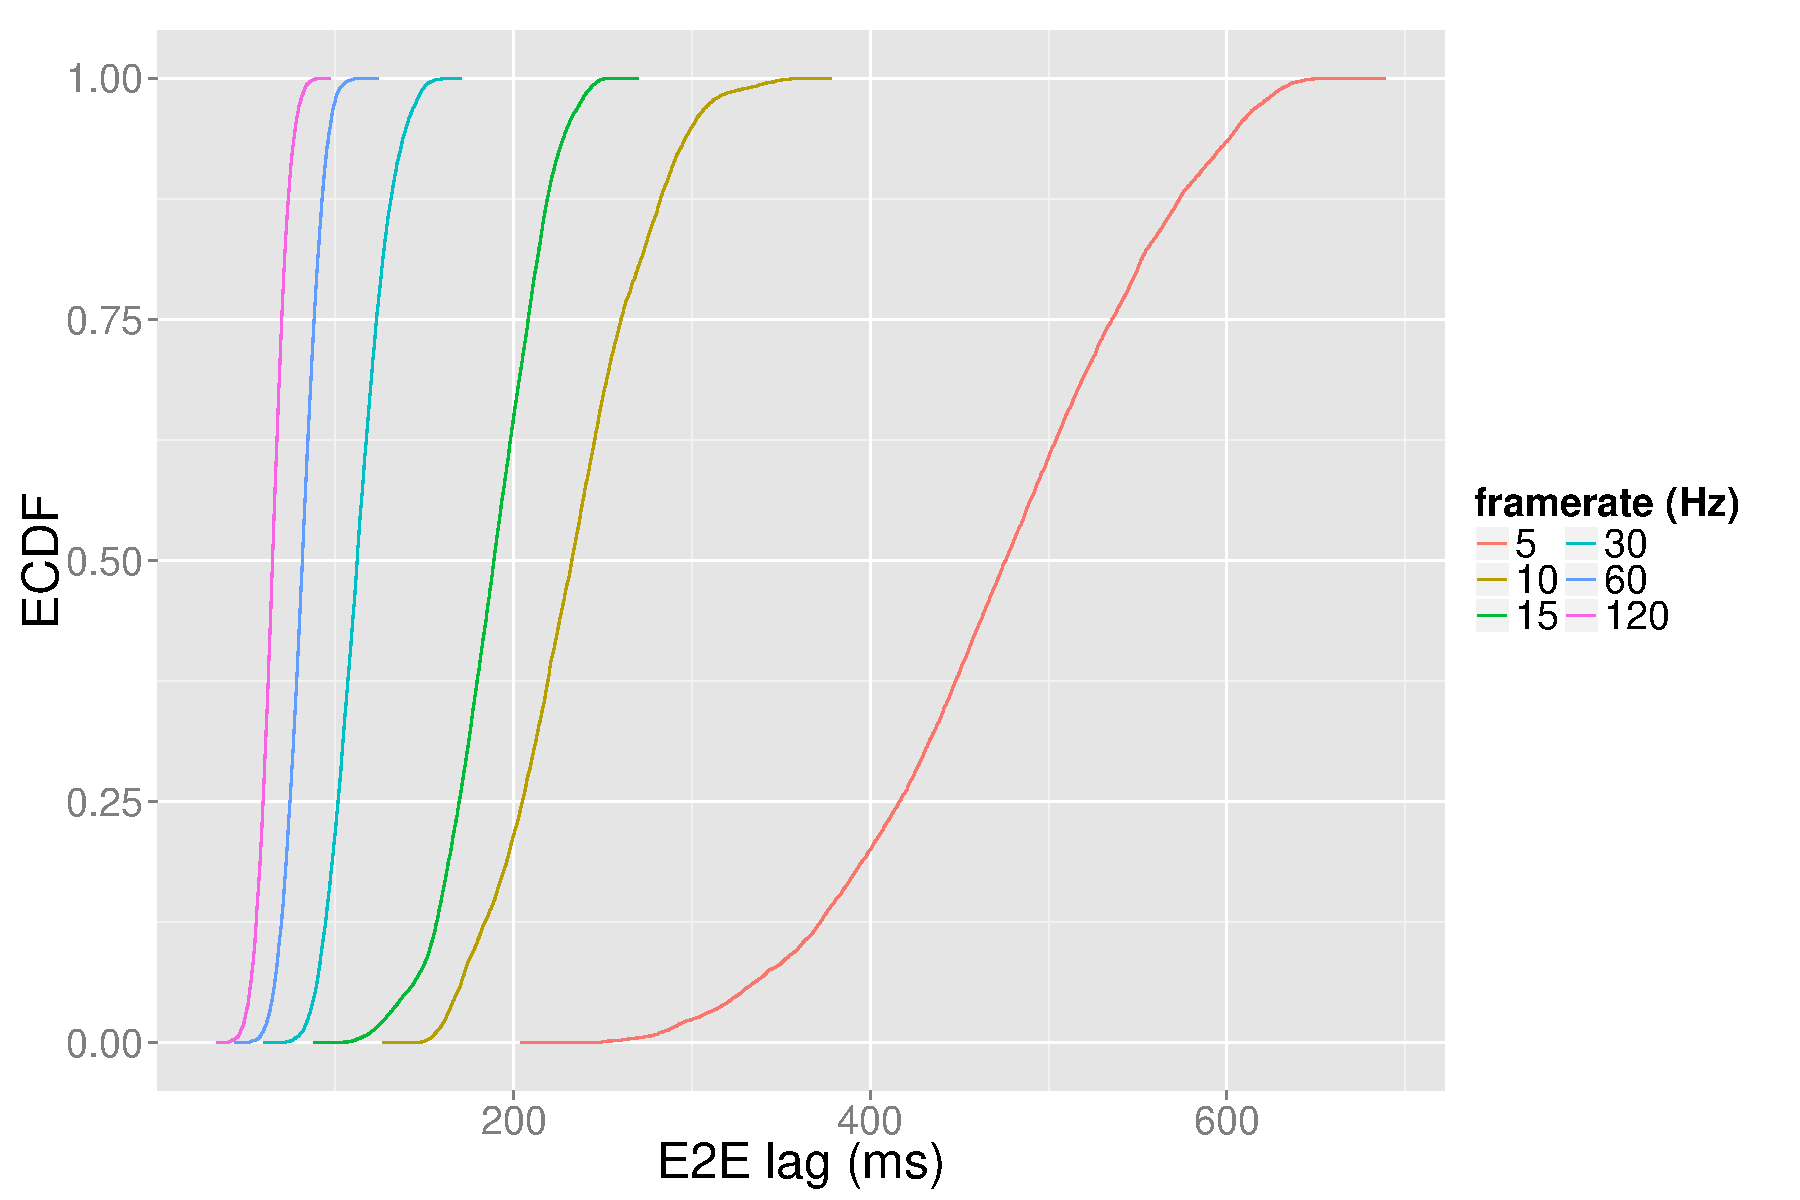
\includegraphics[width=0.7\textwidth]{../../../simulation/visualization/cloudgaming-lag-cdf.pdf}

		Influence of the rendering and streaming framerate on the \gls{E2E} lag in the cloud scenario. The vertical reference line denotes the average server processing time, network round-trip and codec delay $\mu_P+2\mu_D+e+d=\SI{68}{\milli\second}$.
	\end{center}
\end{frame}




\begin{frame}
	\frametitle{Conclusions}

	\begin{itemize}
		\item Expected influence guidelines for future user studies
	\end{itemize}
\end{frame}



\begin{frame}
	\frametitle{Thanks!}

	\Put(130,25){\fcolorbox{black}{white}{\Huge Questions!}}

	\vfill
	Contact: \url{florian.metzger@uni-due.de}\\
	Key fingerprint: \texttt{C98A 32B7 554F C5CC 4E5A  60FB 1CE5 B541 7B20 99C7}
\end{frame}






%%%%%%%%%%%%%%%%%%%%%%%%%%%%%%%%%%%%%%%%%%%%%%%%%%%%%%%%%%%%%%%%%%%%%%%%%%%%%%%%
\appendix
\newcounter{finalframe}
\setcounter{finalframe}{\value{framenumber}}


\begin{frame}
	\frametitle{Backup Slides}
\end{frame}


\begin{frame}
	\frametitle{Static Framerate Figure Backup}

	\begin{center}
		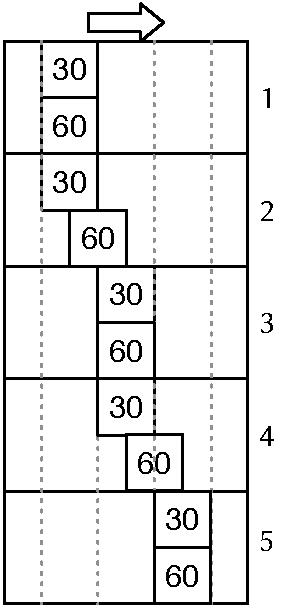
\includegraphics[width=0.25\textwidth]{../../../models/framerate-poster.pdf}
	\end{center}
\end{frame}

\begin{frame}
	\frametitle{Alternate Framerate Animation Backup}

	\begin{center}
		\movie[width=9cm, height=6cm, autostart, repeat, poster]{}{extras/eli5-framerate.mov}\vspace{2mm}
		{\tiny\url{http://hugelol.com/lol/364250}}
	\end{center}
\end{frame}



\begin{frame}
	\frametitle{Simplified Video Game Main Loops}

	\begin{center}
		%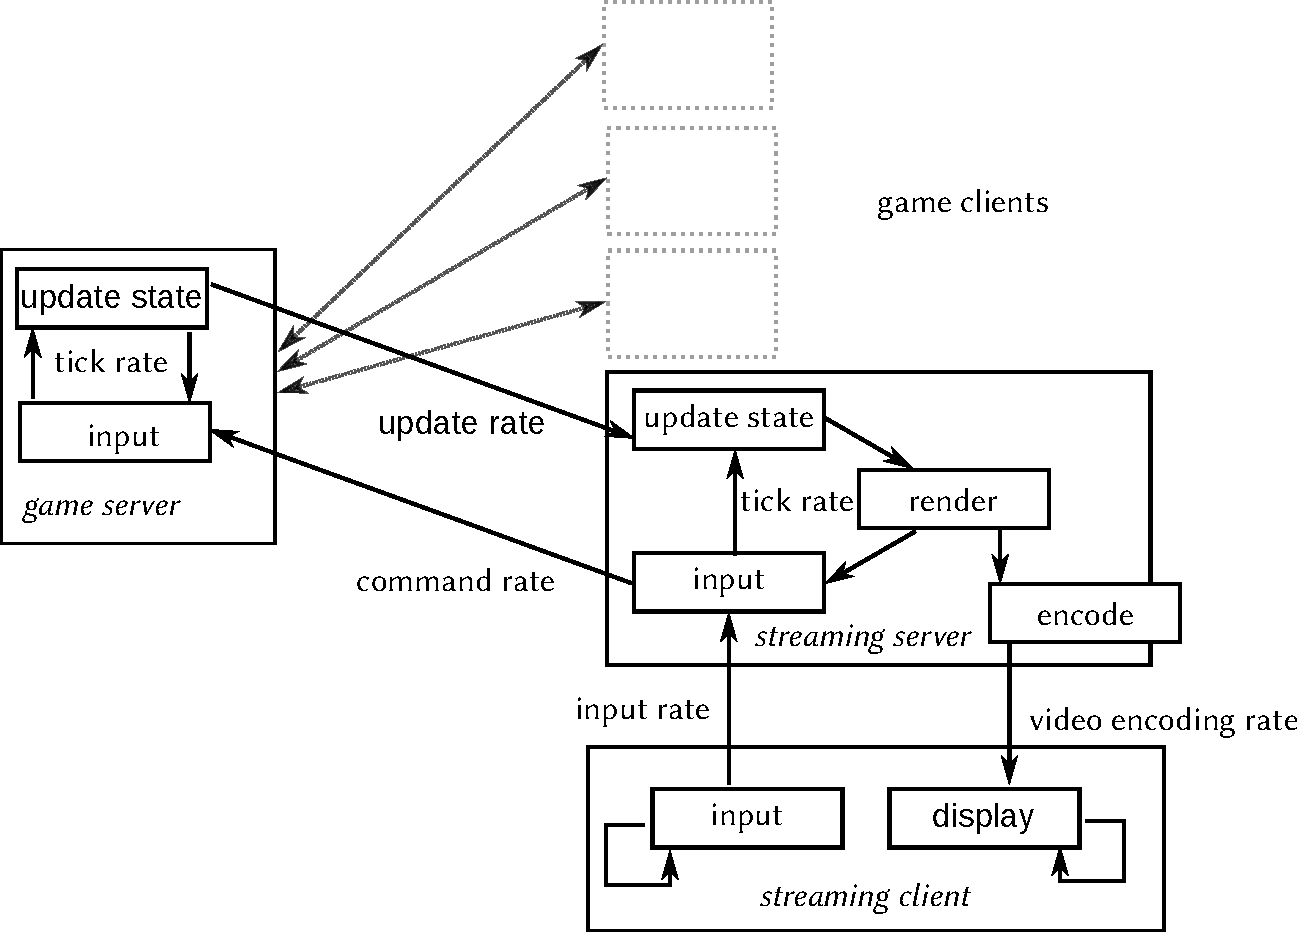
\includegraphics[height=3cm]{../../../models/game-tick-rate-streamed.pdf}

		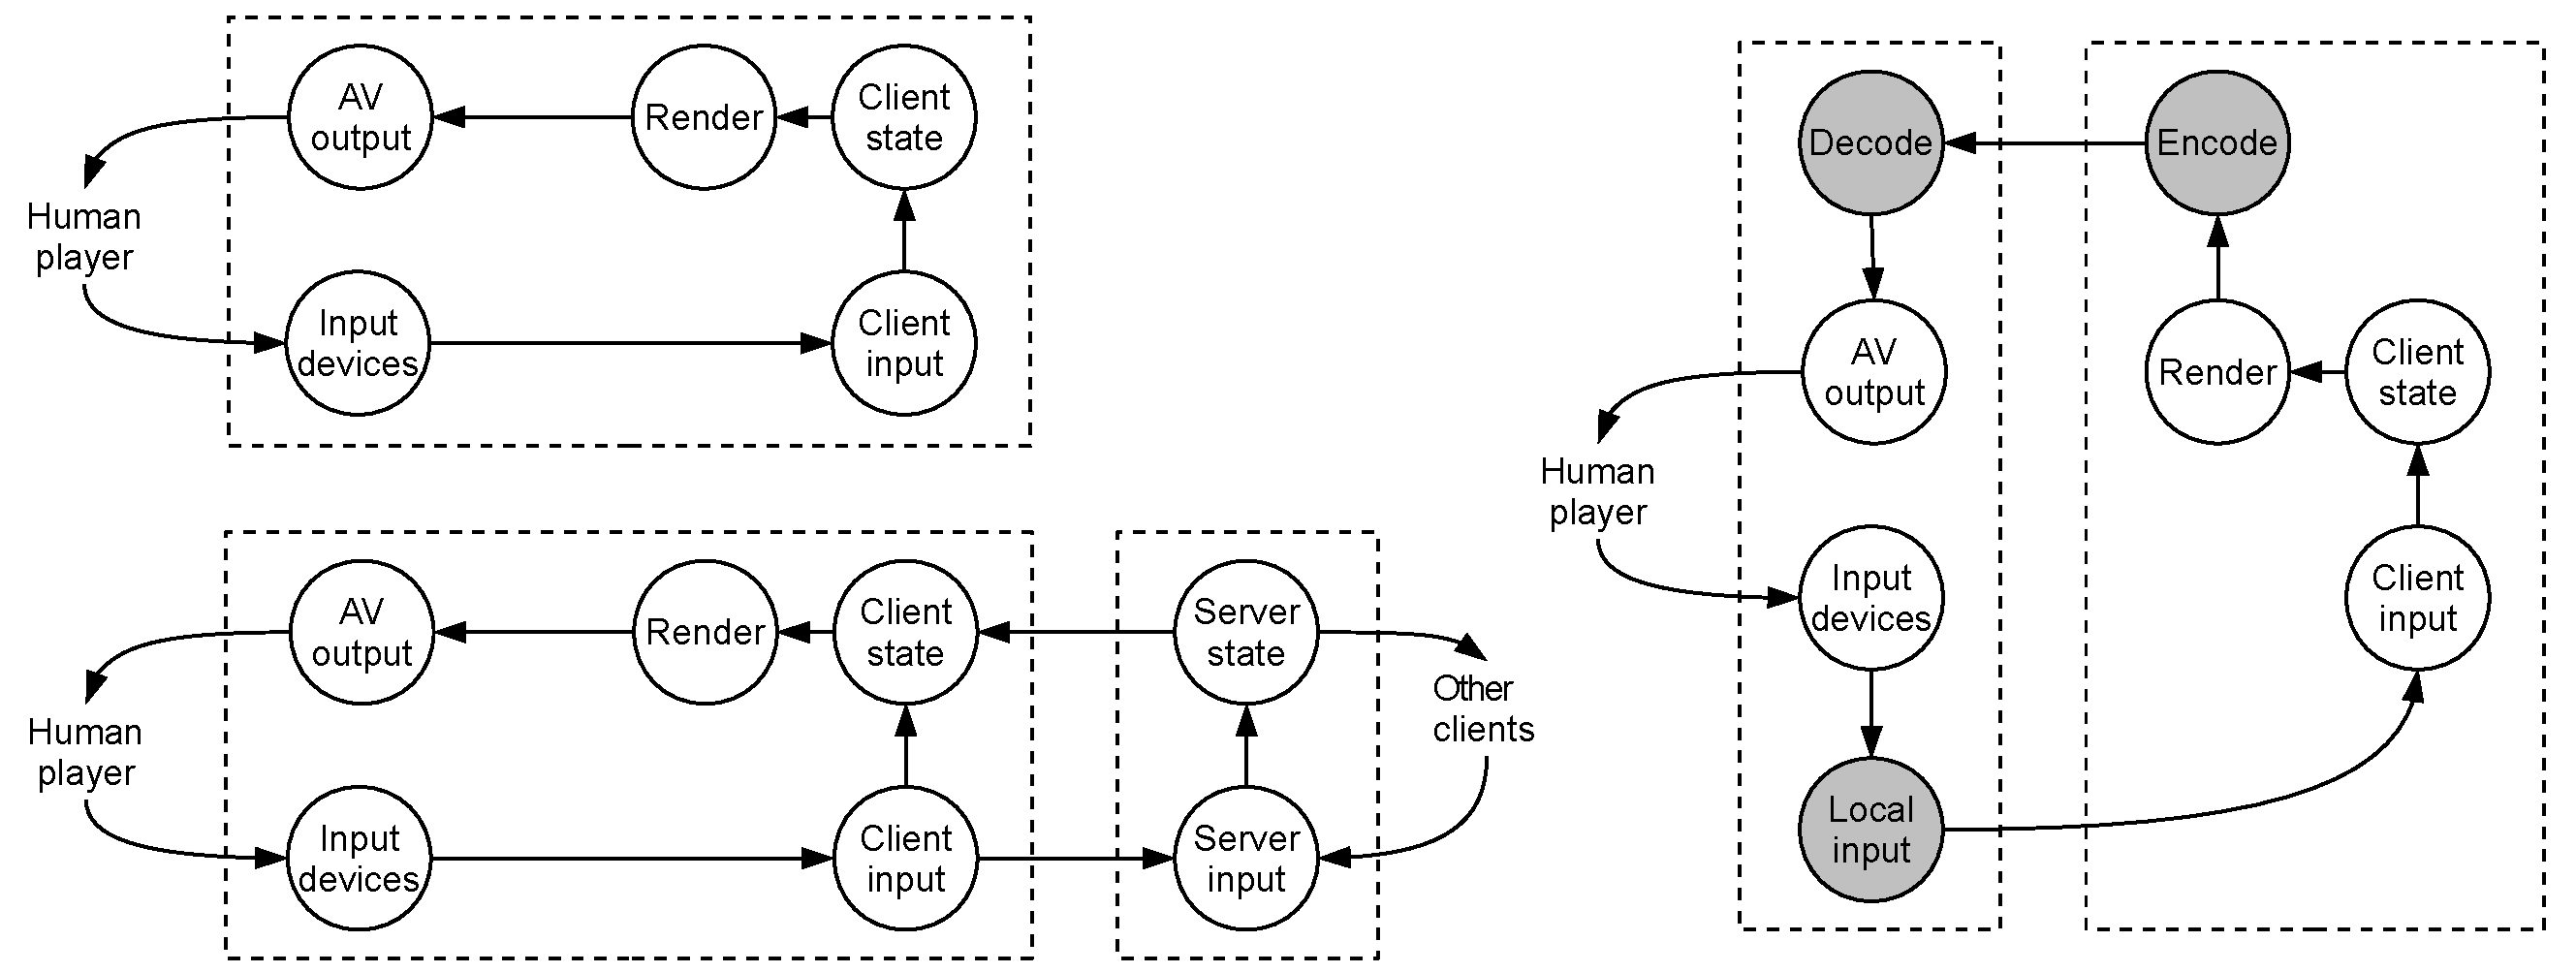
\includegraphics[width=\textwidth]{../../../models/component_interaction_full.pdf}

		{\small \textit{(a)} local game, \textit{(b)} networked game, \textit{(c)} cloud game}
	\end{center}

\end{frame}


\begin{frame}
	\frametitle{Tickrates in Video Games}

	\begin{center}
	Command message rates and client update rates can differ from server tickrates
	{\small
		\begin{tabu}{X[0.45]X}
			\toprule
			\textbf{Video Game} & \textbf{Tickrate} \\
			\midrule
			CS: GO & Configurable \SI{64}{\hertz}/\SI{128}{\hertz} \\
			Battlefield 4 & Configurable \SI{60}{\hertz}/\SI{120}{\hertz}; previously \SI{30}{\hertz} with \SI{10}{\hertz} for state outside of close proximity  \\
			Minecraft & max. \SI{20}{\hertz} \\
			League of Legends & \SI{30}{\hertz} \\
			Dota 2 & \SI{30}{\hertz} \\
			StarCraft II & supposedly either \SI{16}{\hertz} or \SI{32}{\hertz} \\
			Eve Online & \SI{1}{\hertz} \\
%			Project Cars & \SI{600}{\hertz} (Physics), \SI{250}{\hertz} (Input) \\ %https://twitter.com/projectcarsgame/status/551340759858040833
			Overwatch & 60 (client update rate previously was 20) \\
			\bottomrule
		\end{tabu}}

	Note: Values are considered to be unofficial and may be unreliable

	\end{center}

\end{frame}



\begin{frame}[allowframebreaks]
	\frametitle{References}

	\nocite{metzger2016gamesframes,5976180,4591393,4604397,6614351,mollertowards,Claypool:2006:LPA:1167838.1167860,1266180,claypool2007,Bredel:2010:MSR:1944796.1944797,Ivkovic:2015:QMN:2702123.2702432,Ware:1994:ROV:198425.198426,wertheimer1912experimentelle}
	\printbibliography[heading=none, title=none]

\end{frame}

\setcounter{framenumber}{\value{finalframe}}


\end{document}